% Section 02 - Schrodinger problem for dressed quantum Hall system

Our system consist of a two-dimentional free electron gas (2DEG) confined in the $(x,y)$ plane of the three-dimentional coordinate space. In our analysis, the 2DEG is subjected to a stationary magnetic field $\vb{B} = (0,0,B)^{\text{T}}$ which is pointed towards the $z$ axis. In addition, a linearly polarized strong light is applied perpendicular to the 2DEG plane, and we specially tune the frequency of the field $\omega$ such that the optical field behaves as a purely dressing field (unabsorbable). Without limiting the generality we can choose $y$-polorized electric field $\vb{E} = (0,E\sin(\omega t),0)^{\text{T}}$ for the dressing field configuration (Fig.~\ref{fig_1}).
\begin{figure}[b]
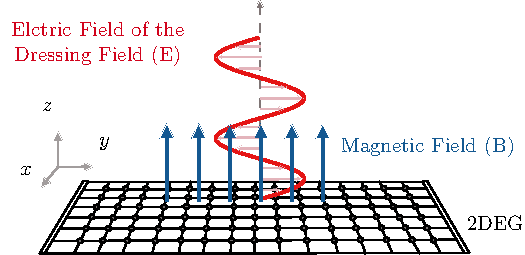
\includegraphics[scale=0.9]{figures/fig_1}
\caption{\label{fig_1} Two-dimensional electron gas (2DEG) confined in the $(x,y)$ plane while both stationary magnetic field $\vb{B}$ and strong dressing field with y-polarized electric field $\vb{E}$ are being applied perpendicular to the surface of 2DEG.}
\end{figure}
Here $B$ and $E$ represent the amplitude of the stationary magnetic field and oscillating electric field respectively.

Using Landau gauge for the stationary magnetic field, we can represent it using vector potential as $\vb{A}_{s} = (-By,0,0)^{\text{T}}$ and choosing Coulomb gauge, the vector potential of the dynamic dressing radiation can be presented as $\vb{A}_{d}(t) = (0,[E/\omega ]\cos(\omega t),0)^{\text{T}}$. These vector potentials are coupled to the momentum of 2DEG as kinetic momentum \cite{mahan00,bruus04} and this leads to the time-dependent Hamiltonian
\begin{equation} \label{eq_1}
  \hat{H}_e(t) = \frac{1}{2m_e}\Big[\hat{\vb{p}} - e\big(\vb{A}_{s}+\vb{A}_{d}(t)\big)\Big]^2,
\end{equation}
where $m_e$ is the effective electron mass and $e$ is the magnitude of the electron charge. $\hat{\vb{p}} = (\hat{p}_x,\hat{p}_y,0)^{\text{T}}$ represents the canonical momentum operator for 2DEG with electron momentum $p_{x,y}$.
The exact solutions for the time-dependent Schrödinger equation $i\hbar \dv{t}\psi = \hat{H}_e(t) \psi$ was already given by Refs. \cite{husmi53,ditt98,dini16} and we can present them as a set of wave functions defined by two quantum numbers $(n,m)$
\begin{equation} \label{eq_2}
  \begin{aligned}
    \psi_{n,m}&(x,y,t)  \\
    & = \frac{1}{\sqrt{L_x}}
    \chi_n\left[y - y_0 - \zeta(t)\right]\\
    & \times
    \text{exp}\bigg(
    \frac{i}{\hbar}\bigg[- \varepsilon_nt
    + p_x x + \frac{eE(y - y_0)}{\omega}\cos(\omega t)\\
    &+
    m_e\dot{\zeta}(t)\big[y - y_0 -\zeta(t)\big] +
    \int_0^{t}dt'L(\zeta,\dot{\zeta},t')\bigg]\bigg),
  \end{aligned}
\end{equation}
where $n \in \mathbb{Z}^{+}_0$ and $m \in \mathbb{Z}$ ; see Appendix A. Here $L_{x,y}$ are dimension of the 2DEG surface, $\hbar$ is the reduced Planck constant, and $y_0 = -p_x/eB$ is the center of the cyclotron orbit along $y$ axis. $\chi_n$ are well known solutions for Schrödinger equation of a stationary quantum harmonic oscillator
\begin{equation} \label{eq_3}
  \chi_n(x) \equiv
   \frac{\sqrt{\kappa}}{\sqrt{2^{n}n!}}
  e^{-\kappa^2 x^2/2}
  \mathcal{H}_n \qty(\kappa x) \quad \text{with}
  \quad
  \kappa = \sqrt{\frac{m_e \omega_0}{\hbar}},
\end{equation}
with eigenvalues given by $\varepsilon_n = \hbar \omega_0 (n + 1/2)$ and $\omega_0 = eB/m_e$ is the cyclotron frequency. Each $n$ value defines the  energy($\varepsilon_n$) of the respective Landau level. The path shift of the driven classical oscillator $\zeta(t)$ is given by
\begin{equation} \label{eq_4}
  \zeta(t) = \frac{eE}{m_e(\omega_0^2 - \omega^2)}\sin(\omega t),
\end{equation}
while the Lagrangian of the classical oscillator $L(\zeta,\dot{\zeta},t)$ can be identified as
\begin{equation} \label{eq_5}
  L(\zeta,\dot{\zeta},t) = \frac{1}{2} m_e\dot{\zeta}^2(t) - \frac{1}{2}m_e\omega_0^2 \zeta^2(t) + eE\zeta(t) \sin(\omega t).
\end{equation}
The exponential phase shifts in Eq.~(\ref{eq_2}) represent the influence done by the stationary magnetic field and strong dressing field. Therefore, we can accept that magneto-transport properties of 2DEG will be renormalized by the magnetic field as well as the dressing field.
